% ============================================================
%  CS 5002 – Project 1 Part 1 Report
% ============================================================
\documentclass[11pt, letterpaper]{article}

% ---- Packages -----------------------------------------------
\usepackage[margin=1in]{geometry}
\usepackage{amsmath, amssymb}
\usepackage{graphicx}
\usepackage{booktabs}
\usepackage{enumitem}
\usepackage{hyperref}
\usepackage{xcolor}
\usepackage{listings}
\usepackage{caption}
\usepackage{float}
\usepackage{parskip}        % space between paragraphs, no indent
\usepackage{titlesec}
\usepackage{fancyhdr}

% ---- Code style ---------------------------------------------
\definecolor{codebg}{RGB}{245,245,245}
\definecolor{codeframe}{RGB}{200,200,200}
\definecolor{keyword}{RGB}{0,100,180}
\definecolor{comment}{RGB}{100,130,100}
\definecolor{string}{RGB}{160,40,40}

\lstset{
  language=Python,
  backgroundcolor=\color{codebg},
  frame=single,
  rulecolor=\color{codeframe},
  basicstyle=\ttfamily\small,
  keywordstyle=\color{keyword}\bfseries,
  commentstyle=\color{comment}\itshape,
  stringstyle=\color{string},
  numbers=left,
  numberstyle=\tiny\color{gray},
  numbersep=8pt,
  breaklines=true,
  captionpos=b,
  showstringspaces=false,
  tabsize=4
}

% ---- Header / Footer ----------------------------------------
\pagestyle{fancy}
\fancyhf{}
\lhead{CS5002 Discrete Structures – Project 1 Part 1}
\rhead{Wanjing Yang 002442139}
\cfoot{\thepage}

% ---- Title block --------------------------------------------
\title{%
  \textbf{CS 5002 – Discrete Structures}\\[4pt]
  \large Project 1 Part 1: Gradient Descent\\[2pt]
  \normalsize Spring 2026
}
\author{ Wanjing Yang \\ NU ID: 002442139}
\date{}

% =============================================================
\begin{document}
\maketitle
\thispagestyle{fancy}

% ---- Table of Contents --------------------------------------
\tableofcontents
\newpage

% =============================================================
\section{Section 2.1 – Gradient Descent on Quadratic Functions}
% =====================================================
\subsection{Background}

We consider the two quadratic functions
\begin{equation}
  f_1(x)=x^2 \qquad \text{and} \qquad f_2(x)=x^2-2x+3.
\end{equation}
Their exact derivatives are
\begin{equation}
  f_1'(x)=2x \qquad \text{and} \qquad f_2'(x)=2x-2.
\end{equation}
A minimum occurs where $f'(x)=0$.  The gradient descent update rule steps
opposite to the gradient:
\begin{equation}
  \boxed{x_{k+1} = x_k - \alpha\,f'(x_k)}
\end{equation}
where $\alpha>0$ is the learning rate.  Iteration stops when
\begin{equation}
  |x_{k+1}-x_k| < \varepsilon
\end{equation}
or the iteration count reaches \texttt{iter\_max}.

\subsection{Part 1 — Basic Test}

\textbf{Parameters:} $x_0=3$, $\alpha=0.1$, $\varepsilon=0.001$,
\texttt{iter\_max}$=1000$.

\begin{table}[H]
\centering
\caption{Gradient descent results for $f_1$ and $f_2$ (basic test).}
\begin{tabular}{lrrrr}
\toprule
Function & $x_0$ & $x^*$ & $f(x^*)$ & Iterations \\
\midrule
$f_1$ & 3 & 0.003714 & 0.000014 & 29 \\
$f_2$ & 3 & 1.003869 & 2.000015 & 27 \\
\bottomrule
\end{tabular}
\end{table}

Both functions converge close to their true minima ($x^*=0$ for $f_1$ and
$x^*=1$ for $f_2$) with a small residual error controlled by $\varepsilon$.

\begin{figure}[H]
  \centering
  \begin{minipage}{0.48\textwidth}
    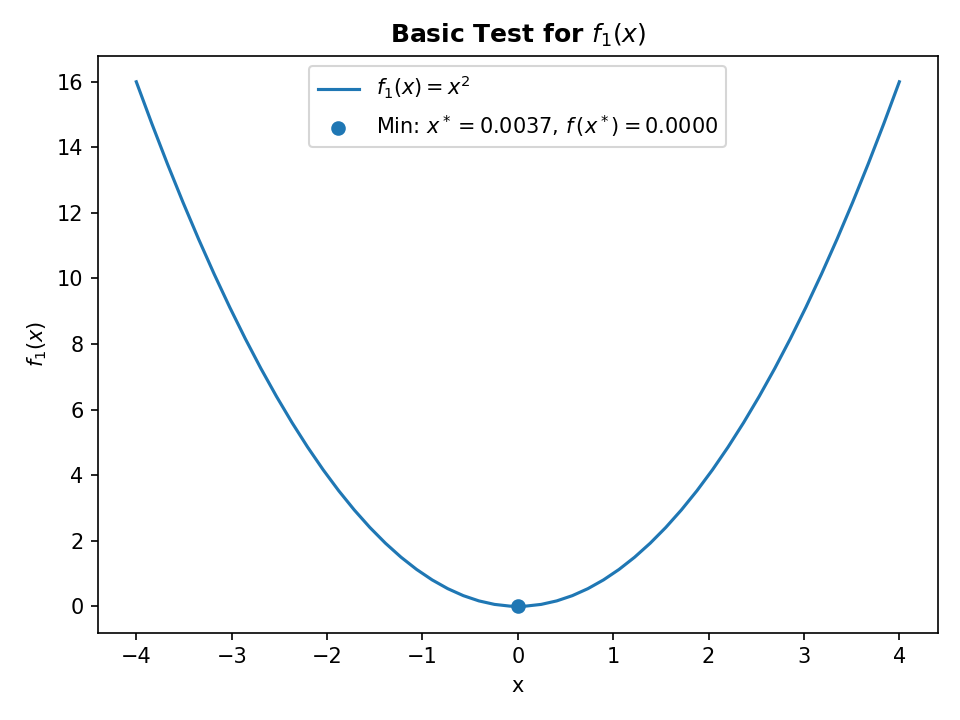
\includegraphics[width=\linewidth]{Basic test for f1.png}
    \caption{GD result on $f_1(x)=x^2$.}
  \end{minipage}\hfill
  \begin{minipage}{0.48\textwidth}
    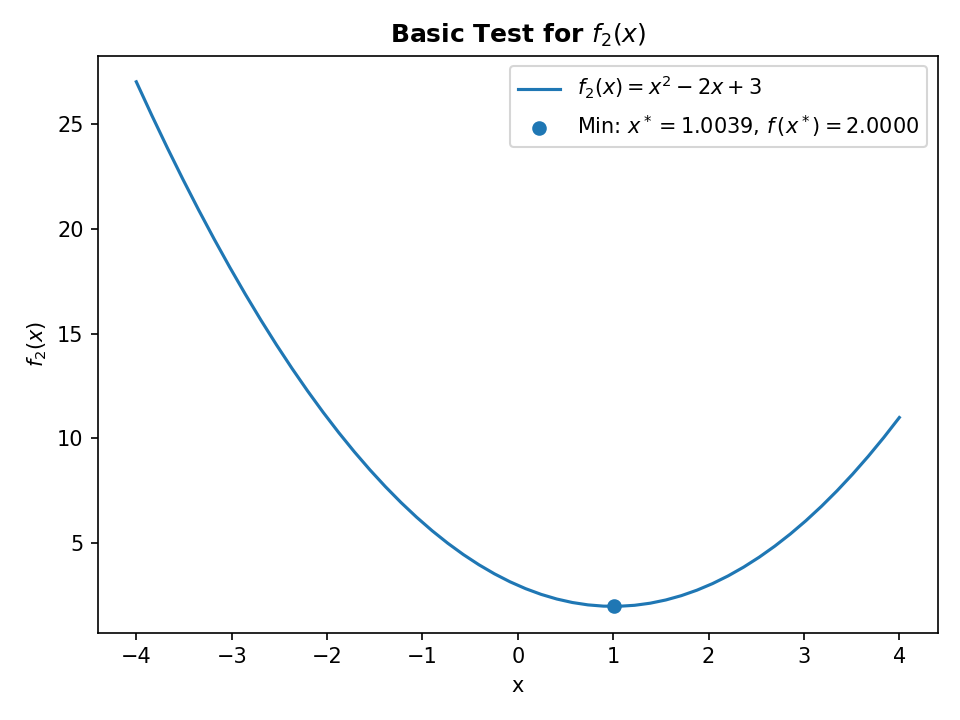
\includegraphics[width=\linewidth]{Basic test for f2.png}
    \caption{GD result on $f_2(x)=x^2-2x+3$.}
  \end{minipage}
\end{figure}

\subsection{Part 2 — Varying $x_0$}

\textbf{Parameters:} $x_0\in\{3,-3\}$, $\alpha=0.1$, $\varepsilon=0.001$,
\texttt{iter\_max}$=1000$.

\begin{table}[H]
\centering
\caption{Effect of changing the starting point $x_0$.}
\begin{tabular}{llrrrr}
\toprule
Function & $x_0$ & $x^*$ & $f(x^*)$ & Iterations \\
\midrule
$f_1$ &  3 &  0.003714 & 0.000014 & 29 \\
$f_1$ & -3 & -0.003714 & 0.000014 & 29 \\
$f_2$ &  3 &  1.003869 & 2.000015 & 27 \\
$f_2$ & -3 &  0.996039 & 2.000016 & 30 \\
\bottomrule
\end{tabular}
\end{table}

Both functions are \textbf{convex} (bowl-shaped), so there is only one global
minimum regardless of where we start.  The starting point $x_0$ affects the
number of iterations but not the final value found.

\subsection{Part 3 — Varying $\alpha$}

\textbf{Parameters:} $x_0=3$, $\alpha\in\{1,\,0.001,\,0.0001\}$,
$\varepsilon=0.001$, \texttt{iter\_max}$=1000$.

\begin{table}[H]
\centering
\caption{Effect of changing the learning rate $\alpha$.}
\begin{tabular}{llrrrr}
\toprule
Function & $\alpha$ & $x^*$ & Iterations & Observation \\
\midrule
$f_1$ & 1      & 3.000000 & 1000 & Diverges / oscillates \\
$f_1$ & 0.001  & 0.498984 &  895 & Slow convergence \\
$f_1$ & 0.0001 & 2.999400 &    0 & Step $<\varepsilon$ immediately \\
$f_2$ & 1      & 3.000000 & 1000 & Diverges / oscillates \\
$f_2$ & 0.001  & 1.498455 &  693 & Slow convergence \\
$f_2$ & 0.0001 & 2.999600 &    0 & Step $<\varepsilon$ immediately \\
\bottomrule
\end{tabular}
\end{table}

\begin{itemize}
  \item $\alpha=1$: too large — the update overshoots and the algorithm
        never converges within \texttt{iter\_max}.
  \item $\alpha=0.001$: valid but slow — many iterations are needed.
  \item $\alpha=0.0001$: too small — the very first step is already smaller
        than $\varepsilon$, so the algorithm terminates at $x_0$ without
        making meaningful progress.
\end{itemize}

\subsection{Part 4 — Varying $\varepsilon$}

\textbf{Parameters:} $x_0=3$, $\alpha=0.1$,
$\varepsilon\in\{0.1,\,0.01,\,0.001\}$, \texttt{iter\_max}$=1000$.

\begin{table}[H]
\centering
\caption{Effect of changing the tolerance $\varepsilon$.}
\begin{tabular}{llrr}
\toprule
Function & $\varepsilon$ & $x^*$ & Iterations \\
\midrule
$f_1$ & 0.1   & 0.322123 &  9 \\
$f_1$ & 0.01  & 0.034588 & 19 \\
$f_1$ & 0.001 & 0.003714 & 29 \\
$f_2$ & 0.1   & 1.335544 &  7 \\
$f_2$ & 0.01  & 1.036029 & 17 \\
$f_2$ & 0.001 & 1.003869 & 27 \\
\bottomrule
\end{tabular}
\end{table}

A looser tolerance (larger $\varepsilon$) terminates earlier with a less
precise result.  A tighter tolerance (smaller $\varepsilon$) requires more
iterations but yields a more accurate minimum.  There is a clear
accuracy–cost trade-off.

% ══════════════════════════════════════════════════════════════════════════════
\section{Section 2.2 — Non-Convex Function $f_3$}

\subsection{Background}

We consider the non-convex function
\begin{equation}
  f_3(x) = \sin(x)+\cos\!\left(\sqrt{2}\,x\right), \quad 0\le x\le 10,
\end{equation}
with exact derivative
\begin{equation}
  f_3'(x) = \cos(x)-\sqrt{2}\,\sin\!\left(\sqrt{2}\,x\right).
\end{equation}
Unlike the quadratics in Section~2.1, $f_3$ has \textbf{multiple local minima}
in $[0,10]$.

\begin{figure}[H]
  \centering
  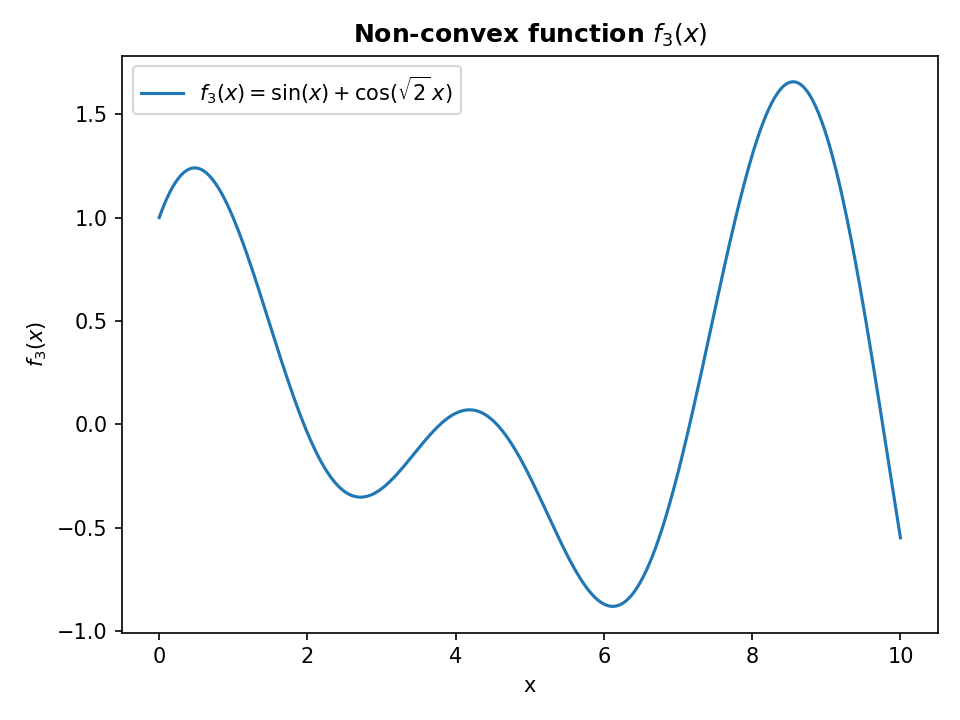
\includegraphics[width=0.65\textwidth]{Non-convex function f3.png}
  \caption{$f_3(x)$ over $[0,10]$, showing multiple local minima.}
\end{figure}

\subsection{Part 2 — Multiple Starting Points}

\textbf{Parameters:} $x_0\in\{1,4,5,7\}$, $\alpha=0.1$,
$\varepsilon=0.0001$, \texttt{iter\_max}$=1000$.

\begin{table}[H]
\centering
\caption{GD on $f_3$ from four different starting points.}
\begin{tabular}{rrrr}
\toprule
$x_0$ & $x^*$ & $f_3(x^*)$ & Iterations \\
\midrule
1 & 2.7156 & -0.3524 & 65 \\
4 & 2.7171 & -0.3524 & 79 \\
5 & 6.1180 & -0.8805 & 49 \\
7 & 6.1190 & -0.8805 & 41 \\
\bottomrule
\end{tabular}
\end{table}

\begin{figure}[H]
  \centering
  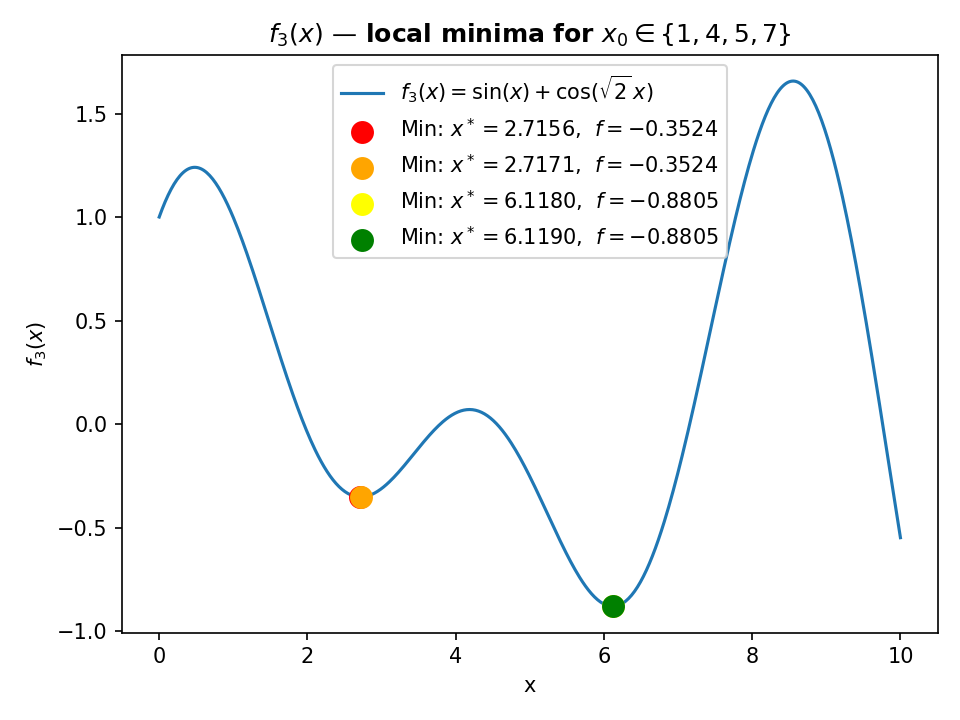
\includegraphics[width=0.65\textwidth]{Local minima for f3.png}
  \caption{Local minima of $f_3$ found from four starting points.}
\end{figure}

Starting points $x_0=1$ and $x_0=4$ both converge to the same local minimum
near $x^*\approx2.72$ (valley A), while $x_0=5$ and $x_0=7$ both converge to
a deeper local minimum near $x^*\approx6.12$ (valley B).  This demonstrates
that for \textbf{non-convex} functions, the starting point $x_0$ determines
\emph{which} local minimum is found — there is no guarantee of reaching the
global minimum.

% ══════════════════════════════════════════════════════════════════════════════
\section{Section 3 — Derivative Approximation}

\subsection{Background}

When the exact derivative is unavailable, we approximate it using the
\textbf{forward finite difference} formula, which follows directly from the
limit definition of the derivative:
\begin{equation}
  f'(x) \approx \frac{f(x+h)-f(x)}{h}, \quad h=10^{-5}.
\end{equation}

\subsection{Accuracy of the Approximation}

\begin{table}[H]
\centering
\caption{Comparison of exact vs.\ approximated derivatives ($h=10^{-5}$).}
\begin{tabular}{llrrr}
\toprule
Function & $x$ & Exact $f'(x)$ & Approx $f'(x)$ & Error \\
\midrule
$f_1$ & $-5$ & $-10.000000$ & $-9.999990$ & $1.00\times10^{-5}$ \\
$f_1$ &  $0$ &   $0.000000$ &  $0.000010$ & $1.00\times10^{-5}$ \\
$f_1$ &  $2$ &   $4.000000$ &  $4.000010$ & $1.00\times10^{-5}$ \\
$f_2$ & $-5$ & $-12.000000$ & $-11.999990$ & $1.00\times10^{-5}$ \\
$f_2$ &  $0$ &  $-2.000000$ &  $-1.999990$ & $1.00\times10^{-5}$ \\
$f_2$ &  $2$ &   $2.000000$ &   $2.000010$ & $1.00\times10^{-5}$ \\
\bottomrule
\end{tabular}
\end{table}

The approximation error is of order $h=10^{-5}$, which is negligible for
practical optimisation purposes.

\subsection{Gradient Descent with Approximate Derivative}

Using the approximated derivative inside gradient descent with $x_0=3$,
$\alpha=0.1$, $\varepsilon=0.001$:

\begin{table}[H]
\centering
\caption{GD with approximated derivative vs.\ exact derivative.}
\begin{tabular}{lrrr}
\toprule
Function & $x^*$ (approx) & $x^*$ (exact) & Difference \\
\midrule
$f_1$ & 0.003714 & 0.003714 & $\sim 0$ \\
$f_2$ & 1.003869 & 1.003869 & $\sim 0$ \\
\bottomrule
\end{tabular}
\end{table}

\begin{figure}[H]
  \centering
  \begin{minipage}{0.48\textwidth}
    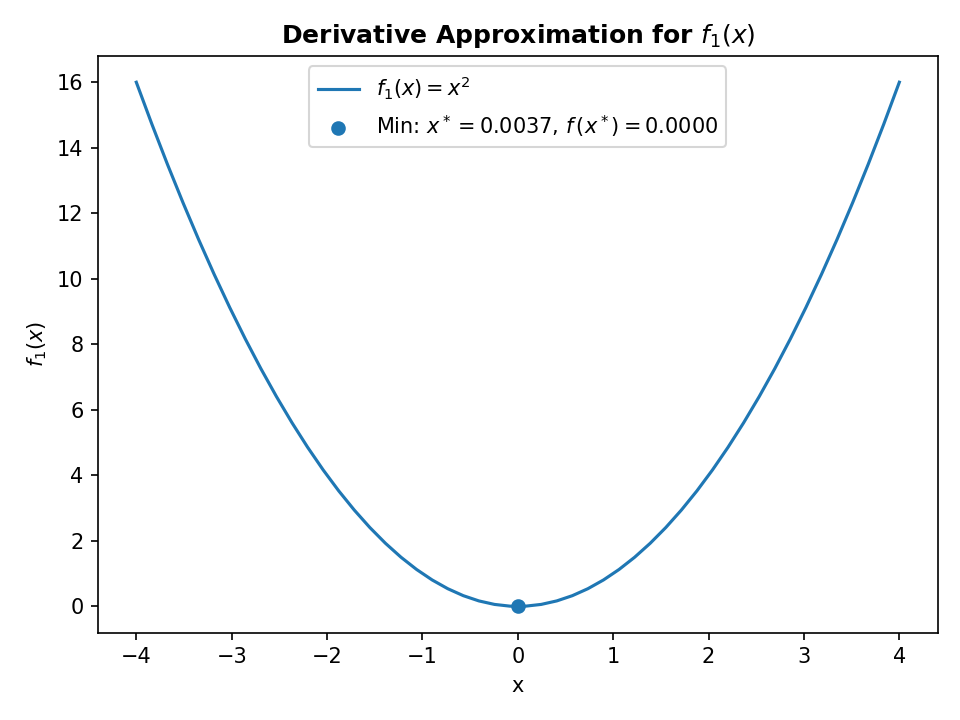
\includegraphics[width=\linewidth]{Derivative Approximation for f1.png}
    \caption{GD with approximated derivative on $f_1$.}
  \end{minipage}\hfill
  \begin{minipage}{0.48\textwidth}
    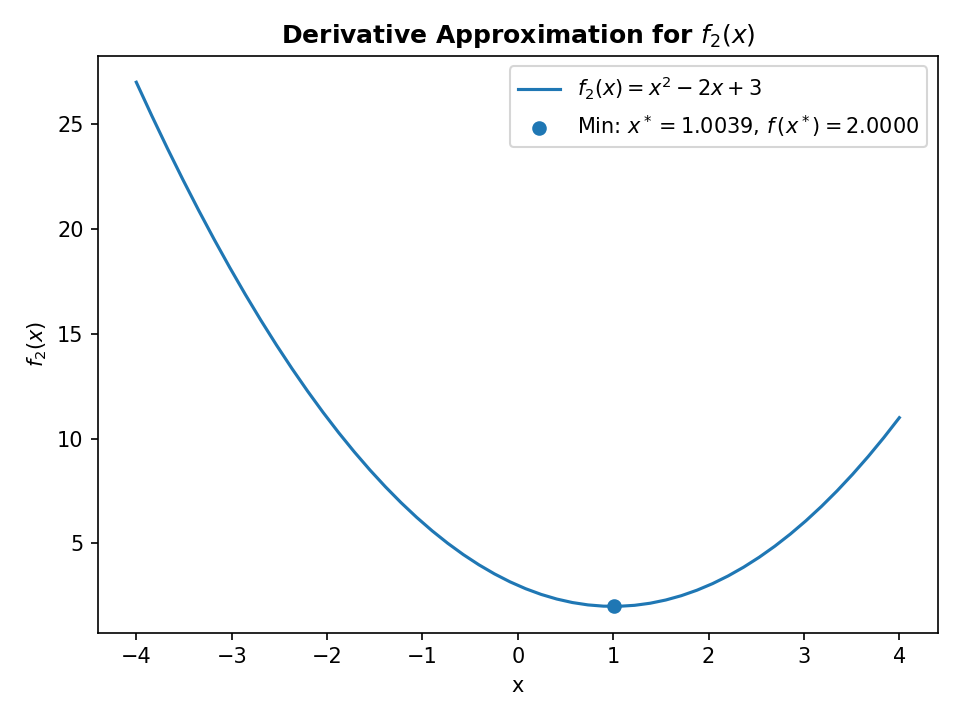
\includegraphics[width=\linewidth]{Derivative Approximation for f2.png}
    \caption{GD with approximated derivative on $f_2$.}
  \end{minipage}
\end{figure}

The results are essentially identical to those obtained with the exact
derivative.  The $O(h)$ approximation error is far smaller than the stopping
tolerance $\varepsilon=0.001$ and therefore has no visible effect on the
converged solution.

% ══════════════════════════════════════════════════════════════════════════════
\section{Section 4 — Gradient Descent for Functions of Two Variables}

\subsection{Background}

We extend gradient descent to a function of two variables $f(x,y)$.  Both
variables are updated simultaneously at each iteration:
\begin{equation}
  x_{k+1} = x_k - \alpha\,\frac{\partial f}{\partial x}(x_k,y_k), \qquad
  y_{k+1} = y_k - \alpha\,\frac{\partial f}{\partial y}(x_k,y_k).
\end{equation}
Convergence is declared when \emph{both} coordinate steps fall below
$\varepsilon$:
\begin{equation}
  |x_{k+1}-x_k|<\varepsilon \quad \text{and} \quad |y_{k+1}-y_k|<\varepsilon.
\end{equation}
The partial derivatives are approximated using the same finite difference idea:
\begin{equation}
  \frac{\partial f}{\partial x}(x_0,y_0)\approx\frac{f(x_0+h,\,y_0)-f(x_0,y_0)}{h}.
\end{equation}

\subsection{Results on $f(x,y)=x^2+y^2$}

\textbf{Parameters:} $x_0=y_0=3$, $\alpha=0.1$, $\varepsilon=0.001$,
$h=10^{-5}$, \texttt{iter\_max}$=1000$.

\begin{table}[H]
\centering
\caption{2D gradient descent result on $f(x,y)=x^2+y^2$.}
\begin{tabular}{rrrr}
\toprule
$x^*$ & $y^*$ & $f(x^*,y^*)$ & Iterations \\
\midrule
0.003709 & 0.003709 & 0.000028 & 29 \\
\bottomrule
\end{tabular}
\end{table}

\begin{figure}[H]
  \centering
  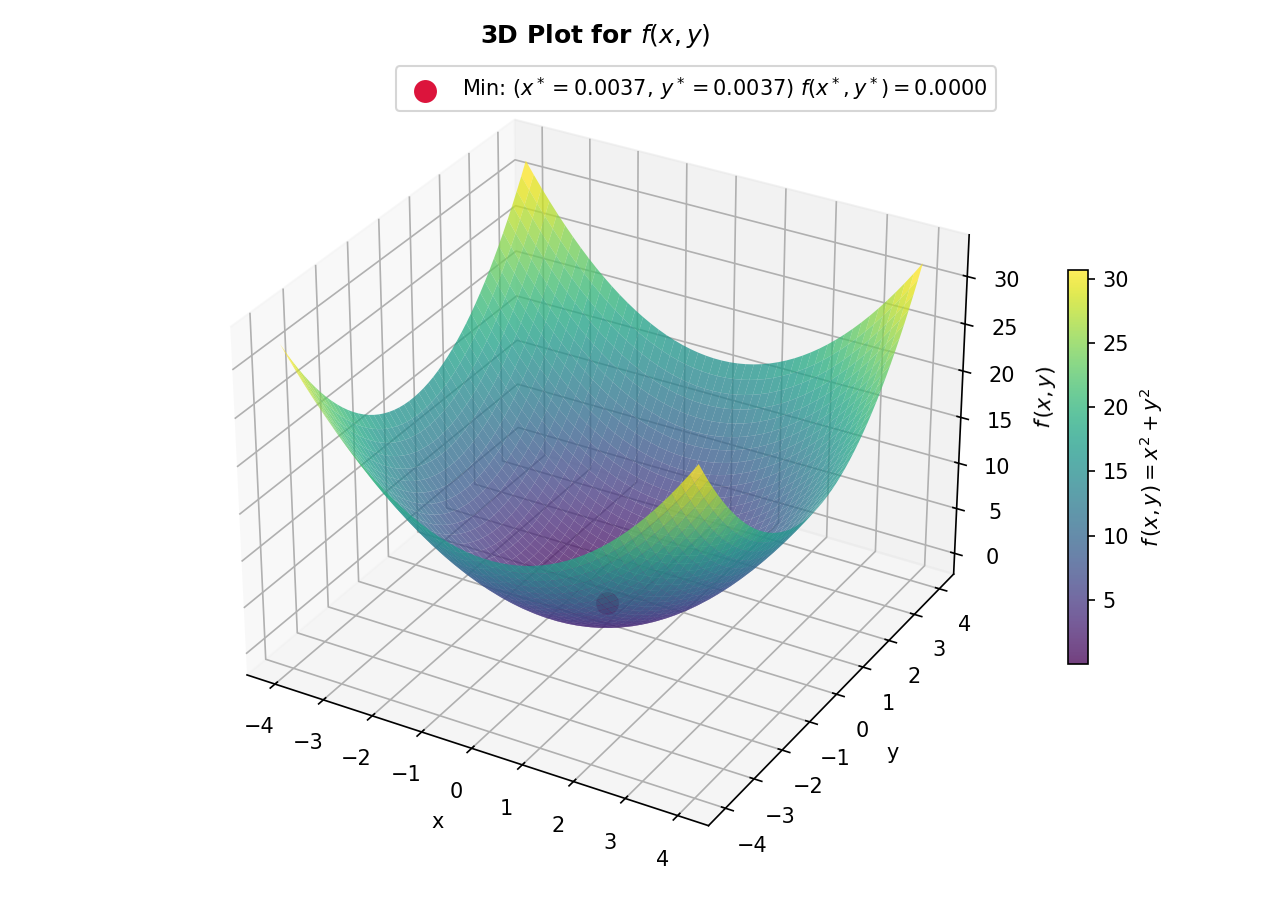
\includegraphics[width=0.65\textwidth]{3D Plot for f(x,y).png}
  \caption{3D surface of $f(x,y)=x^2+y^2$ with the gradient descent minimum
           marked in red.}
\end{figure}

The algorithm converges to $(x^*,y^*)\approx(0.0037,\,0.0037)$, very close to
the true global minimum at $(0,0)$.  The result confirms that the 2D extension
using approximate partial derivatives works correctly.

% ══════════════════════════════════════════════════════════════════════════════
\section{Conclusion}

This project implemented and analyzed gradient descent across four settings.
The key findings are:

\begin{itemize}
  \item \textbf{Convex functions:} the starting point $x_0$ does not affect the
        final minimum, only the number of iterations.
  \item \textbf{Non-convex functions:} $x_0$ determines which local minimum is
        found; there is no guarantee of finding the global minimum.
  \item \textbf{Learning rate $\alpha$:} too large causes oscillation/divergence;
        too small causes premature stopping or very slow convergence.
  \item \textbf{Tolerance $\varepsilon$:} controls the accuracy–cost trade-off;
        a tighter tolerance gives a more precise result at greater computational cost.
  \item \textbf{Derivative approximation:} forward finite differences with
        $h=10^{-5}$ introduce an error of order $10^{-5}$, negligible relative
        to typical stopping tolerances.
  \item \textbf{2D extension:} the framework generalises naturally to two
        variables using approximate partial derivatives, with identical
        hyperparameter trade-offs.
\end{itemize}


\end{document}